%\pagenumbering{arabic}
%\setcounter{page}{1}

\chapter{Introduzione al GIS}

\begin{wrapfigure}{O}{0.5\columnwidth}
	\begin{centering}
		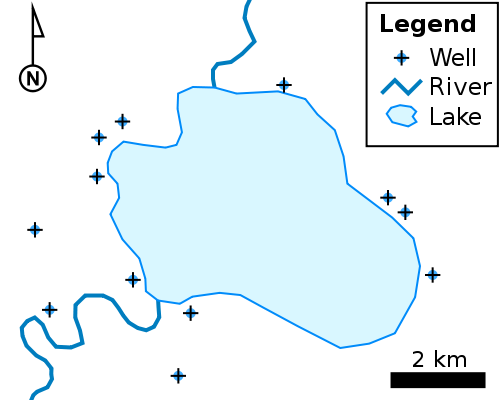
\includegraphics[scale=0.35]{img/500px-Simple_vector_map}
		\par
	\end{centering}
	\caption{{\small\label{fig:Una-semplice-mappa}Una semplice mappa vettoriale, che usa tutti i tre elementi delle geometrie: i punti vengono usati per rappresentare i pozzi, le linee per schematizzare i fiumi e un poligono descrive il lago.}}
	\vspace{-10pt}
\end{wrapfigure}

Per definizione, un \emph{Sistema Informativo Geografico} (SIT) o \emph{Geographic Information System} (GIS) in inglese, è un \emph{sistema informatico per l'acquisizione, conservazione, analisi e visualizzazione di dati geografici}. Viene definito sistema in quanto costituito da un insieme di componenti (hardware, software ed umane) che interagiscono tra loro, per dare vita alla caratteristica principale di un GIS: gestire dati geografici o georeferenziati, ovvero dati relativi ad elementi od oggetti della superficie terrestre la cui posizione è definita da un insieme (non necessariamente una coppia) di coordinate. Rispetto ad una rappresentazione puramente geometrica degli oggetti, il GIS deve memorizzare i dati descrittivi (\emph{attributi}) dei singoli oggetti reali, in tabelle: ogni riga si riferisce ad un singolo oggetto e ogni colonna ad un singolo attributo. Ogni GIS è dunque basato su un modello del mondo reale definito per la specifica applicazione; tale concetto verrà meglio definito successivamente.

\section{Il modello dei dati
%\footnote{Geographic information system. (2009, August 26). In Wikipedia, The Free Encyclopedia. Retrieved 15:10, August 26, 2009, from http://en.wikipedia.org/w/index.php?title=Geographic\_information\_system\&oldid=310176131}
}

	Un sistema GIS è una formalizzazione degli oggetti presenti nella realtà; per descrivere correttamente gli oggetti reali distribuiti sulla superficie terrestre, è indispensabile che siano caratterizzati da:
	
	\begin{description}
		\item [{geometria}] riproduce la forma degli oggetti e viene ricondotta a tre elementi (schematizzati in fig. \ref{fig:Una-semplice-mappa}), definiti da \emph{vettori}:

			\begin{description}
				\item [{punti}] sono entità adimensionali usate per elementi geografici che possono essere espressi da un singolo punto (può essere il caso della sommità di una collina o di una montagna, o della posizione di un albero); il concetto di informazione puntuale è strettamente legato al rapporto tra estensione dell'elemento ed estensione dell'area in analisi\footnote{Ad esempio, se si sta analizzando la posizione degli alberi monumentali su un'estensione di 4 ettari, ogni albero sarà simboleggiato da un punto; invece, se si sta analizzando l'area coperta da alberi monumentali in un giardino di \unit{\meter\squared} di area, ogni albero sarà rappresentato non più da un punto, ma da un'area.};
				\item [{linee}] o polilinee, sono entità monodimensionali utilizzate per descrivere strutture lineari (ad esempio fiumi, strade, ferrovie, ecc.); è altresì valido per le linee il concetto di rapporto tra estensione dell'elemento e dell'area;
				\item [{poligoni}] o aree, sono usati per descrivere entità che ricoprono una certa area dell'estensione terrestre, come laghi, confini di parchi naturali, città, palazzi, ecc.; dall'informazione poligonale è possibile ricavare sia la misura di un perimetro che quella dell'area coperta dal poligono stesso. 
			\end{description}
			
			Due considerazioni importanti a proposito della geometria:
		
			\begin{itemize}
				\item Ognuna di queste geometrie è definita, all'interno del database geografico, da una riga, ovvero da un \emph{record} di dati, che descrive i suoi attributi.
				\item Le diverse geometrie possono essere comparate tra loro, o messe in rapporto ad altri elementi di differenti geometrie; ade esempio, è possibile ottenere facilmente un confronto tra l'area di ciascun lago, così come un elenco di tutti i picchi montuosi a meno di 10 km dal centro del lago.
			\end{itemize}

		\item [{topologia}] è l'insieme delle informazioni che riguardano le relazioni spaziali reciproche tra i diversi elementi della geometria, come la \emph{connessione}, l'\emph{adiacenza} o l'\emph{inclusione}. Permette ad esempio di specificare se una linea è connessa ad un'altra o se semplicemente si sovrappongono senza comunicare (schematizzazione di due strade che possono intersecarsi a formare un incrocio o sovrapporsi in un cavalcavia). I dati vettoriali generati dalle geometrie possono essere gestiti in maniera tale che siano rispettate le \emph{regole topologiche}, come ad esempio ``i poligoni non devono sovrapporsi''. I dati vettoriali individuati dalle geometrie e nel rispetto delle regole topologiche, possono rappresentare astrazioni più o meno complesse della superficie terrestre, come ad esempio l'elevazione del terreno, rappresentata tramite un insieme di poligoni (triangoli) adiacenti i cui vertici sono disposti nelle tre dimensioni dello spazio.
		
		\item [{attributi}] sono dati che descrivono gli oggetti reali, associati alle rappresentazioni geometriche di quegli oggetti nel GIS. Per esempio, una database che descrive dei laghi può contenere informazioni aggiuntive collegate alle semplici informazioni geografiche sulla geometria dei laghi, come la loro profondità massima, il grado di salinità, la presenza di sostanze inquinanti,ecc.. Queste informazioni possono essere utilizzate per generare una mappa tematica con l'obiettivo di descrivere un particolare attributo del set di dati, tra quelli citati sopra; ad esempio, i laghi possono essere colorati in funzione del livello di inquinamento.

	\end{description}

\section{La rappresentazione dei dati}
	Nel GIS esistono due tipi di rappresentazione dei dati, ``vettoriale'' (\emph{vector} in inglese) e ``raster'' (un esempio in fig. \ref{fig:A-sinistra,-rappresentazione}). Nella rappresentazione \textbf{vettoriale}, introdotta precedentemente, ogni punto è definito da una coppia di coordinate (se questo punto è parte di una linea o di un poligono, si avrà un insieme di coppie di coordinate, che individuano i vari punti, connessi tra loro con segmenti retti che formano la rappresentazione grafica dell'elemento). Generalmente i punti alle estremità di una linea vengono definiti \emph{nodi}, mentre quelli intermedi \emph{vertici}.\\ Nella rappresentazione \textbf{raster}, l'area considerata è suddivisa in un insieme di celle, solitamente di forma quadrata, in ciascuna delle quali viene registrato l'attributo (o categoria) presente, sotto forma di valore numerico, come si vede in fig.~\ref{fig:Listato-di-un-raster}.\\
	
	\begin{figure}
		\centering
			\begin{minipage}[c][1\totalheight][t]{0.5\columnwidth}

				\begin{center} \texttt{north: 15} \end{center}
				\begin{center} \texttt{south: 0} \end{center}
				\begin{center} \texttt{east: 15} \end{center}
				\begin{center} \texttt{west: 0} \end{center}
				\begin{center} \texttt{rows: 15} \end{center}
				\begin{center} \texttt{cols: 15} \end{center}

				\begin{spacing}{0.3}
					\begin{center} \texttt{3 3 1 1 1 1 1 1 1 3 3 3 3 3 3} \par\end{center}
					\begin{center} \texttt{3 3 1 1 1 1 1 1 1 3 3 3 3 3 3} \par\end{center}
					\begin{center} \texttt{3 3 1 1 1 1 1 1 1 3 3 3 3 3 3} \par\end{center}
					\begin{center} \texttt{3 3 1 1 1 1 1 1 1 3 3 3 3 3 3} \par\end{center}
					\begin{center} \texttt{2 2 2 2 2 2 2 2 2 2 2 2 2 2 2} \par\end{center}
					\begin{center} \texttt{2 2 2 2 2 2 2 2 2 2 2 2 2 2 2} \par\end{center}
					\begin{center} \texttt{2 2 2 2 2 2 2 2 2 2 2 2 2 2 2} \par\end{center}
					\begin{center} \texttt{3 3 1 1 1 1 1 1 1 1 1 1 1 3 3} \par\end{center}
					\begin{center} \texttt{3 3 1 1 1 1 1 1 1 1 1 1 1 3 3} \par\end{center}
					\begin{center} \texttt{3 3 1 1 1 1 1 1 1 1 1 1 1 3 3} \par\end{center}
					\begin{center} \texttt{3 3 1 1 1 1 1 1 1 1 1 1 1 3 3} \par\end{center}
					\begin{center} \texttt{3 3 1 1 1 1 1 1 1 1 1 1 1 3 3} \par\end{center}
					\begin{center} \texttt{3 3 3 3 3 3 3 3 3 3 3 3 3 3 3} \par\end{center}
					\begin{center} \texttt{3 3 3 3 3 3 3 3 3 3 3 3 3 3 3} \par\end{center}
					\begin{center} \texttt{3 3 3 3 3 3 3 3 3 3 3 3 3 3 3} \par\end{center}
				\end{spacing}
			\end{minipage}
		\caption{{\small\label{fig:Listato-di-un-raster}Listato di un raster esportato in formato testuale. Idealmente, in questo listato ogni ``cella'' della griglia è rappresentata da un numero, il cui valore definisce la caratteristica della cella.}}
	\end{figure}

	\begin{figure}
		\centering
		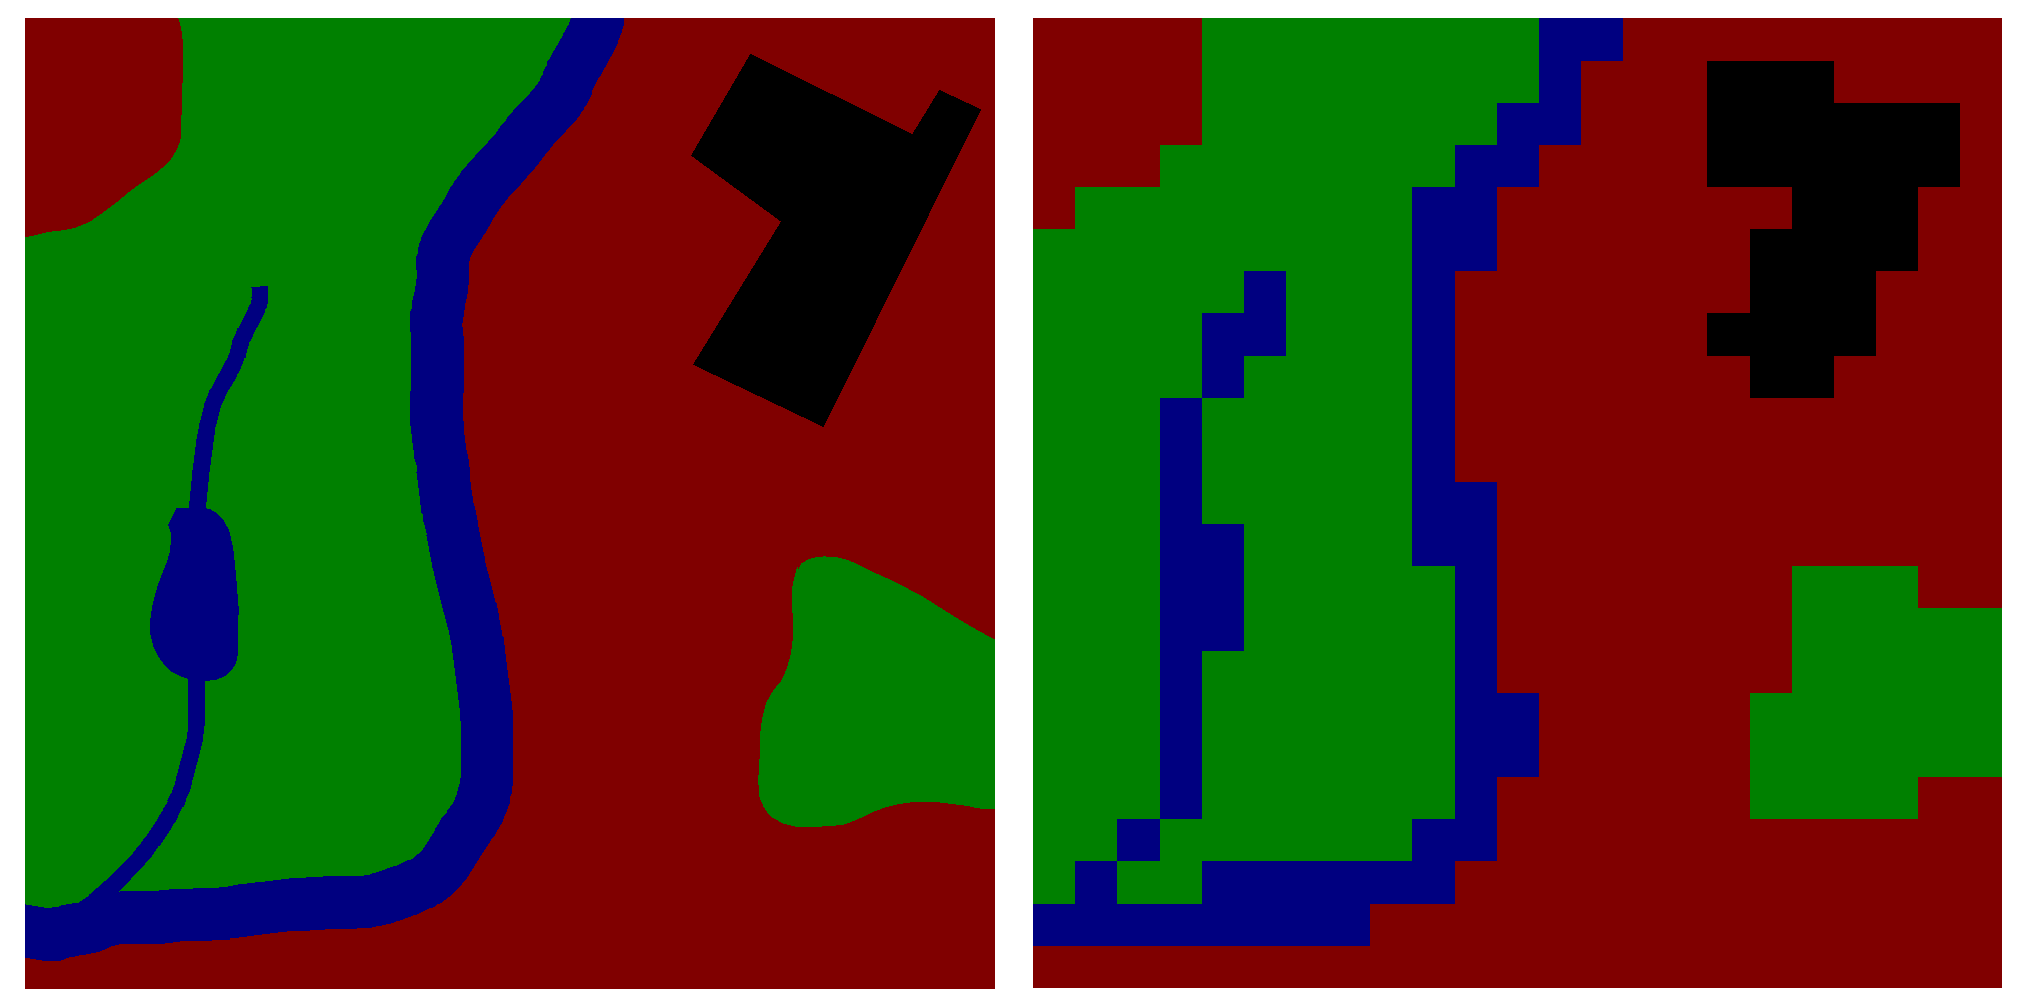
\includegraphics[scale=0.1]{img/Raster_vector_gis}
		\caption{{\small\label{fig:A-sinistra,-rappresentazione}A sinistra, rappresentazione di dati vettoriali, a destra gli stessi dati informato raster.}}
	\end{figure}
	
	Essenzialmente è un raster ogni tipo di immagine digitale costituita da una griglia di informazioni, divisa quindi in celle che definiscono una struttura di righe e colonne. Chiunque abbia familiarità con la fotografia digitale riconosce nel \emph{pixel} la minima unità dell'immagine digitale e quindi l'elemento essenziale della griglia; un insieme di pixel da origine ad un'immagine, differente per questo da un dato di tipo vettoriale. Anche un'immagine raster rappresenta un'astrazione della realtà, perché ogni pixel è colorato in funzione della zona che rappresenta. La risoluzione di un'immagine raster è data dalla dimensione della sua cella in unità del suolo. Le immagini aeree, le ortofoto o le immagini satellitari sono tipi di raster comunemente utilizzati in software GIS, con l'obiettivo di fornire un'immagine dettagliata del territorio, che poi verrà digitalizzata ``disegnando'' su di essa una rappresentazione schematica vettoriale.  Altre tipologie di raster possono contenere informazioni selettive: per esempio, ogni pixel può essere colorato in funzione della sua altitudine (in questo caso si ha un modello di elevazione digitale o \emph{DEM}); altri raster possono contenere informazioni sulla riflessione della luce secondo particolari lunghezze d'onda (dati \emph{LANDSAT}), o secondo la temperatura. Le celle --- pixel --- che costituiscono le immagini possono contenere quindi vari tipi di informazioni sotto forma di diversi colori. È possibile realizzare tali tipologie di raster grazie a delle convenzioni che definiscono una certa scala di colori per rappresentare ben determinate tipologie di informazioni, ad esempio la nota RGB (\emph{red}, \emph{green}, \emph{blue} --- rosso, verde, blu). All'interno di file raster è anche possibile che siano presenti pixel vuoti, rappresentanti porzioni di territorio per le quali il dato in analisi non è disponibile; tali pixel prendono spesso il nome di \emph{null}. I dati raster vengono memorizzati in diversi formati, a partire da una struttura standard sotto forma di file (nel caso di TIF, JPEG, ecc.) fino a grandi quantità di dati raster binari (BLOB) immagazzinati in un sistema di gestione di un database relazionale (RDBMS), in un'impostazione simile a quella di dati vettoriali\footnote{Un insieme di dati archiviati in un database, se opportunamente gestiti, permettono generalmente una gestione più veloce dei dati raster, ma richiedono la registrazione di milioni di \emph{record} all'interno del database (approssimativamente uno per ogni pixel).}.
